\documentclass{beamer}
\mode<presentation>
\usetheme{Madrid}
\usecolortheme{crane}

\usepackage{tikz}
\usepackage{epic}
\usepackage{qtree}
\usepackage{linguex}
\usepackage[normalem]{ulem}
\usepackage{tikz-dependency}
\usepackage{tikzsymbols}

\usepackage{verbatim}
\usepackage{url}
\usepackage{xcolor} % See documentation PDF at http://www.ctan.org/pkg/xcolor
\definecolor{darkgreen}{rgb}{0,0.3,0}
\definecolor{lightgrey}{rgb}{0.65,0.65,0.65}

\newcommand{\remph}[1]{\textbf{\color{red} #1}}

\newcommand{\code}[1]{{\color{darkgreen}\texttt{#1}}}
\newcommand{\detail}[1]{{\color{lightgrey}\small{}#1}}

\title[LT2222 lecture 0]{LT2222 Machine learning for NLP: intro, Winter 2021}
\subtitle{Lecture 0: Introduction; formal foundations}
\author[Sayeed]{Asad Sayeed\\{\small with some material from {\tt https://github.com/jonsafari/lt1}}}
\institute[Gothenburg]{University of Gothenburg}
\date{}

\setbeamertemplate{navigation symbols}{}

\newcommand{\placard}[1]{
  \begin{frame}
    \begin{center}
      \huge
      \textbf{#1}
    \end{center}
  \end{frame}
}

\newcommand{\pagestep}[2]{
  \begin{frame}[t]
    \begin{minipage}[t][0.26\textheight][t]{\textwidth}
      \begin{center}
        \huge
        \textbf{#1}
      \end{center}
    \end{minipage}
    
    \begin{minipage}[t][0.7\textheight][c]{\textwidth}
      \begin{center}
        \includegraphics[height=0.83\textheight]{#2}
      \end{center}
    \end{minipage}
  \end{frame}
}

\newcommand{\pagestepalt}[2]{
  \begin{frame}[t]
    \begin{minipage}[t][0.26\textheight][t]{\textwidth}
      \begin{center}
        \huge
        \textbf{#1}
      \end{center}
    \end{minipage}
    
    \begin{minipage}[t][0.7\textheight][c]{\textwidth}
      #2
    \end{minipage}
  \end{frame}
}

%% \newcommand{\pagestepaltfragile}[2]{
%%   \begin{frame}[fragile][t]
%%     \begin{minipage}[t][0.26\textheight][t]{\textwidth}
%%       \begin{center}
%%         \huge
%%         \textbf{#1}
%%       \end{center}
%%     \end{minipage}
    
%%     \begin{minipage}[t][0.7\textheight][c]{\textwidth}
%%       #2
%%     \end{minipage}
%%   \end{frame}
%% }


\begin{document}
\makeatletter
\setbeamertemplate{footline}
{
  \leavevmode%
  \hbox{%
  \begin{beamercolorbox}[wd=.333333\paperwidth,ht=2.25ex,dp=1ex,center]{author in head/foot}%
    \usebeamerfont{author in head/foot}\insertshortauthor\expandafter\beamer@ifempty\expandafter{\beamer@shortinstitute}{}{~~(\insertshortinstitute)}
  \end{beamercolorbox}%
  \begin{beamercolorbox}[wd=.333333\paperwidth,ht=2.25ex,dp=1ex,center]{title in head/foot}%
    \usebeamerfont{title in head/foot}\insertshorttitle
  \end{beamercolorbox}%
  \begin{beamercolorbox}[wd=.333333\paperwidth,ht=2.25ex,dp=1ex,right]{date in head/foot}%
    \usebeamerfont{date in head/foot}\insertshortdate{}\hspace*{2em}
%    \insertframenumber{} / \inserttotalframenumber\hspace*{2ex} 
    \insertframenumber{}\hspace*{2ex}
    \hspace*{6ex}
  \end{beamercolorbox}}%
  \vskip0pt%
}
\makeatother


\begin{frame}
  \titlepage
\end{frame}


\pagestepalt{Welcome! Today's agenda:}{
  \begin{enumerate}
  \item A lot of boring review
  \item Format and topics of the course
  \item Administrative details
  \end{enumerate}
}

\placard{Part 1: Some boring review\ldots}

\pagestepalt{Statistical approaches to Natural Language Processing are ubiquitous.}{
  \begin{center}
    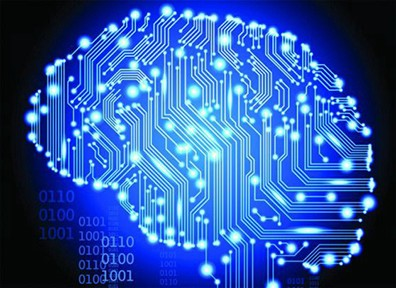
\includegraphics[width=0.5\textwidth]{circuitbrain.jpg}\\
    {\small\it Something that statistical NLP is not.}
  \end{center}
}

\placard{It's easy to think of statistical NLP in the consumer market\ldots or is it?}

\pagestepalt{The ubiquity of statistical NLP}{
  \begin{itemize}
  \item Most internet search-related services (especially so if you include information retrieval).\pause
  \item Popular question-answering systems on your smartphones, e.g., Siri, Cortana.\pause
  \item Basically: any language technology that must deal with highly variable input involves statistical NLP
    in practice --- and that's practically all of them worth talking about.
  \end{itemize}
}

\pagestepalt{But what is statistical NLP?}{
  \begin{itemize}
  \item Catch-all term for the use of \alert{predictive} and/or \alert{discriminative} techniques in accomplishing
    human-language tasks, such that\pause
    \begin{itemize}
    \item the predictions and classifications are not explicitly
      ``hard-coded'' but based on implicit discovery of relationships
      inside the data.\pause
    \item that discovery takes place based on some kind of
      machine-learning technique, often very simple.\pause
    \end{itemize}
  \item Statistical relationships are often used in co-operation with
    ``formal'' approaches, where the underlying linguistic logic is
    made ``explicit''.\pause
  \item Language \alert{science} (e.g. psycholinguistics,
    sociolinguistics) often also uses statistical NLP techniques.
  \end{itemize}\pause
  \begin{center}
    \textbf{Let's illustrate what this really means\ldots} (you saw this last semester\ldots)
  \end{center}
}

\placard{Q: Does language have anything to do with the weather?}

\placard{A: Yes. But first\ldots}

\pagestepalt{\ldots a tongue-twister in English.}{
  \begin{center}
    \Large How much wood could a woodchuck chuck if a woodchuck could
    chuck wood?
  \end{center}\pause
  One possible answer:
  \begin{center}
    \Large As much wood as a woodchuck could chuck. 
  \end{center}
}

\pagestepalt{Can we calculate how \alert{likely} that answer is?}{
  \pause That depends \ldots on what you mean by ``likely''.\pause\\ To
  estimate the likelihood of an answer (in the form of a sentence),
  you need:
  \begin{itemize}
  \item An evidentiary basis.
    \\$\Rightarrow$ in modern \alert{statistical} natural language processing,
    we use large \alert{corpora}. \pause 
  \item A theory that connects the evidence to the likelihood you're
    trying to estimate.  \pause
    \begin{itemize}
    \item Assume sentences are made of words.  
    \item So the probability of a sentence might have something 
      to do with the probability of the words in the sentence.
    \end{itemize}\pause
  \item A means to combine the pieces of evidence.\\
    $\Rightarrow$ if words matter, then we need a \alert{theory} of sentence
    structure from words.
  \end{itemize}
}

\pagestepalt{Why do we want a likelihood?}{
%  \textcolor{blue}{[Solicit answers from students.]}\\ \pause
  Consider natural language processing systems in real life. E.g., machine 
  translation:
  \begin{itemize}
  \item Translate ``How much wood \alert{could} a woodchuck chuck?'' to French.
    \begin{itemize}
    \item The word ``could'': possibility in French expressible with 
      two different grammatical forms ({\it ``peut''/``pourrait''}).
    \item Choose better one {\it in context}.
    \item Hard to do over all words deterministically $\leftarrow$
      years of effort to create the ``rules'', but never succeed.
    \end{itemize}
  \item Countless other applications: such as answering a question\ldots.
  \end{itemize}
}

\pagestepalt{So how do we get the evidence?}{
  Count words.
  \begin{center}
    \Large how much wood could a woodchuck chuck if a woodchuck could
    chuck wood ?
  \end{center}
  Assume that this is our corpus. Total number of words: 14 (incl. the ``?'').
%  \\ \textcolor{blue}{[Get students to follow along.]}\pause
  \only<2>{\vspace{-0.75cm}\begin{columns}[T]
      \begin{column}{0.5\textwidth}
        \begin{center}
          \small
          \begin{tabular}{c|c}
            word type & token count \\
            \hline
            a & 2 \\
            chuck & 2 \\
            could & 2 \\
            how & 1 \\
            if & 1 \\
          \end{tabular}
        \end{center}
      \end{column}
      \begin{column}{0.5\textwidth}
        \begin{center}
          \small
          \begin{tabular}{c|c}
            word type & token count \\
            \hline
            much & 1 \\
            wood & 2 \\
            woodchuck & 2 \\
            ? & 1 \\
          \end{tabular}
        \end{center}
      \end{column}
  \end{columns}}
  \only<3>{\vspace{-0.75cm}\begin{columns}[T]
      \begin{column}{0.5\textwidth}
        \begin{center}
          \small
          \begin{tabular}{c|c|c}
            word type & token count & \alert{p(word)}\\
            \hline
            a & 2 & 0.14\\
            chuck & 2 & 0.14 \\
            could & 2 & 0.14 \\
            how & 1 & 0.07\\
            if & 1 & 0.07 \\
          \end{tabular}
        \end{center}
      \end{column}
      \begin{column}{0.5\textwidth}
        \begin{center}
          \small
          \begin{tabular}{c|c|c}
            word type & token count & \alert{p(word)} \\
            \hline
            much & 1 & 0.07\\
            wood & 2 & 0.14 \\
            woodchuck  &2 & 0.14 \\
            ? & 1 & 0.07 \\
          \end{tabular}
        \end{center}
      \end{column}
  \end{columns}
  Then calculate probability per \alert{type} of word as count/14.
  }


  %% \only<2>{\begin{center}
  %%   \begin{tabular}{c|c|c}
  %%     word & count & \alert{p(word)}\\
  %%     \hline
  %%     a & 2 & 0.14\\
  %%     chuck & 2 & 0.14 \\
  %%     could & 2 & 0.14 \\
  %%     how & 1 & 0.07\\
  %%     if & 1 & 0.07 \\
  %%   \end{tabular}
  %%   \begin{tabular}{c|c|c}
  %%     word & count & \alert{p(word)} \\
  %%     \hline
  %%     much & 1 & 0.07\\
  %%     wood & 2 & 0.14 \\
  %%     woodchuck 2 & & 0.14 \\
  %%     ? & 1 & 0.07 \\
  %%   \end{tabular}
  %% \end{center}
  %% Then calculate probability per \alert{type} of word as count/14.
  %% }
}

\pagestepalt{Calculate the probability of expressions.}{
  \vspace{-1cm}
  \begin{columns}[T]
    \begin{column}{0.5\textwidth}
      \begin{center}
        \small
        \begin{tabular}{c|c|c}
          word type & token count & \alert{p(word)}\\
          \hline
          a & 2 & 0.14\\
          chuck & 2 & 0.14 \\
          could & 2 & 0.14 \\
          how & 1 & 0.07\\
          if & 1 & 0.07 \\
        \end{tabular}
      \end{center}
    \end{column}
    \begin{column}{0.5\textwidth}
      \begin{center}
        \small
        \begin{tabular}{c|c|c}
          word type & token count & \alert{p(word)} \\
          \hline
          much & 1 & 0.07\\
          wood & 2 & 0.14 \\
          woodchuck  &2 & 0.14 \\
          ? & 1 & 0.07 \\
        \end{tabular}
      \end{center}
    \end{column}
  \end{columns}
  The \alert{joint probability} of multiple words: how likely they are to occur
  in the same text.
  \begin{block}{}
    $p(w_1,w_2,\ldots) = p(w_1)p(w_2)\ldots$
  \end{block}
  Calculate some joint probabilities:
% \textcolor{blue}{[student activity]}:
  \begin{itemize}
    \item $p($if,woodchuck$)=$ \only<2>{\alert{0.07 x 0.14 = 0.01} }
    \item $p($wood,woodchuck$)=$ \only<2>{\alert{0.14 x 0.14 = 0.02}}
    \item $p($how,could,a$)=$ \only<2>{\alert{0.07 x 0.14 x 0.14 = 0.001}}
  \end{itemize}
}

\pagestepalt{Calculating the probability of expressions.}{
  \vspace{-1cm}
  \begin{columns}[T]
    \begin{column}{0.5\textwidth}
      \begin{center}
        \small
        \begin{tabular}{c|c|c}
          word type & token count & \alert{p(word)}\\
          \hline
          a & 2 & 0.14\\
          chuck & 2 & 0.14 \\
          could & 2 & 0.14 \\
          how & 1 & 0.07\\
          if & 1 & 0.07 \\
        \end{tabular}
      \end{center}
    \end{column}
    \begin{column}{0.5\textwidth}
      \begin{center}
        \small
        \begin{tabular}{c|c|c}
          word type & token count & \alert{p(word)} \\
          \hline
          much & 1 & 0.07\\
          wood & 2 & 0.14 \\
          woodchuck  &2 & 0.14 \\
          ? & 1 & 0.07 \\
        \end{tabular}
      \end{center}
    \end{column}
  \end{columns}
  Now we can calculate the joint probability of our answer.
  \begin{center}
    \Large As much wood as a woodchuck could chuck. 
  \end{center}
  \begin{itemize}
  \item $p($as,much,wood,as,a,woodchuck,could,chuck$)$ = \pause \alert{0 x \ldots}\pause
  \item Uh oh: there's no ``as'' in our probability table. \\
    $\Rightarrow$ we will get to missing items soon.\pause
  \item So, try $p($much,wood,a,woodchuck,could,chuck$)$ = \\ \pause \alert{0.07 x 0.14 x 0.14 x 0.14 x 0.14 x 0.14  = 3.76e-05}
  \end{itemize}
}

\pagestepalt{Words come in an order.}{
  Calculating the joint probability of \alert{unigrams} (single words):
  is it a good \alert{model}?\pause \\
  Backwards\ldots
  \begin{center}
    \Large chuck could woodchuck a as wood much as
  \end{center}
  \ldots is not an English sentence. \pause
  \begin{itemize}
  \item Joint unigram probability: the same, no matter what, as ``as much wood as a woodchuck could chuck''.\pause
  \item We definitely don't want that to be true.  So our theory must include
    sequences.
  \end{itemize}
}

\placard{And this is what language has to do with the weather.}

\pagestepalt{What was the weather like two years ago in Holland?}{
  Average temperature at Amsterdam Schiphol:\\
  \begin{flushright}
    \begin{tabular}{|c|}
      \hline
      18.11.2014 \\
      {\Huge 8 C} \\
      \hline
   \end{tabular}
  \end{flushright}
}

\pagestepalt{And what was it the day before that?}{
  Average temperature at Amsterdam Schiphol:\\
  \begin{flushright}
    \begin{tabular}{|c|}
      \hline
      17.11.2014 \\
      {\Huge 10 C} \\
      \hline
    \end{tabular}
    \begin{tabular}{|c|}
      \hline
      18.11.2014 \\
      {\Huge 8 C} \\
      \hline
    \end{tabular}
  \end{flushright}
}

\pagestepalt{And before that?}{
  Average temperature at Amsterdam Schiphol:\\
  \begin{flushright}
    \begin{tabular}{|c|}
      \hline
      16.11.2014 \\
      {\Huge 9 C} \\
      \hline
    \end{tabular}
    \begin{tabular}{|c|}
      \hline
      17.11.2014 \\
      {\Huge 10 C} \\
      \hline
    \end{tabular}
    \begin{tabular}{|c|}
      \hline
      18.11.2014 \\
      {\Huge 8 C} \\
      \hline
    \end{tabular}
  \end{flushright}
}


\placard{It's as though we know something about the next day from the
  previous days!}

\placard{But how many days do we need?}

\pagestepalt{Surely not to the beginning of the Earth!}{
  Average temperature at Amsterdam Schiphol:\\
  \begin{flushright}
    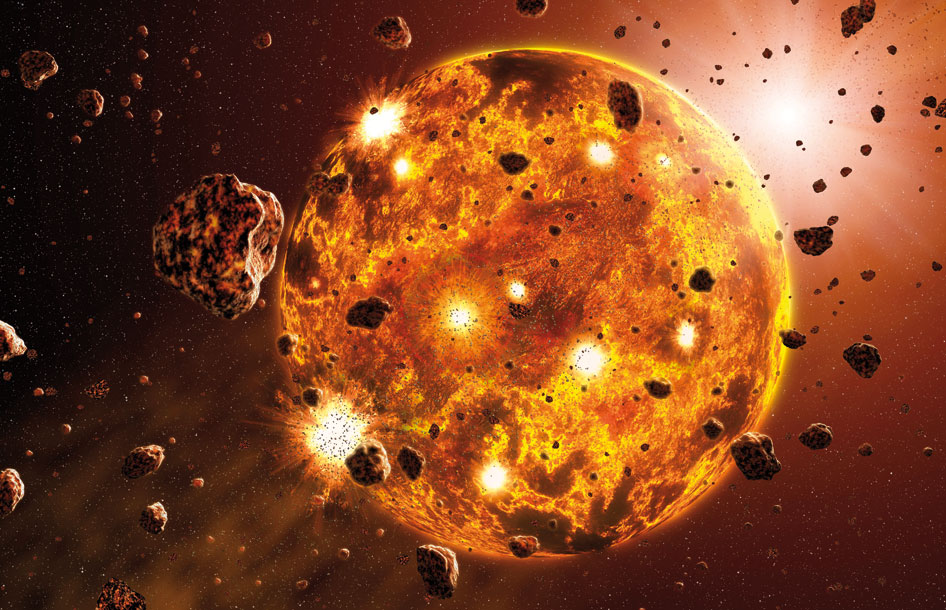
\includegraphics[width=0.3\textwidth]{../images/formation.jpg}
    {\Huge\ldots}
    \begin{tabular}{|c|}
      \hline
      16.11.2014 \\
      {\Huge 9 C} \\
      \hline
    \end{tabular}
    \begin{tabular}{|c|}
      \hline
      17.11.2014 \\
      {\Huge 10 C} \\
      \hline
    \end{tabular}
    \begin{tabular}{|c|}
      \hline
      18.11.2014 \\
      {\Huge 8 C} \\
      \hline
    \end{tabular}
  \end{flushright}
}

\pagestepalt{We have expectations about changes.}{
  We know that yesterday is a good clue about today. \\
  Temperatures in Amsterdam in 2014:
  \begin{center}
    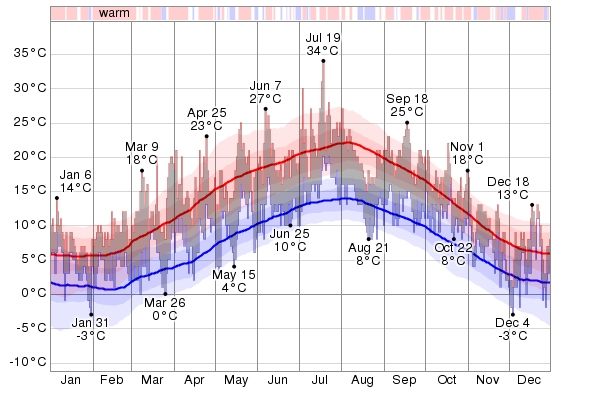
\includegraphics[width=0.70\textwidth]{../images/amstemp.png}
  \end{center}
}

\pagestepalt{The daily temperature is a \alert{Markov process}.}{
  Let $T_d=$ temperature $T$ on day $d$.\\
  We can represent the probability conditionally.
  \begin{block}{Probability of today's temperature \only<1>{given universe}\only<2->{\alert{given 2 previous days}}}
    $p(T_d|T_{d-1},T_{d-2},\ldots,T_{d-\infty})$ \only<2->{\alert{$\approx p(T_d|T_{d-1},T_{d-2})$}}
  \end{block}\pause
  But we only need a few days to give us a trend. So we make a 
  \alert{Markov assumption}.\\ \pause
  Then we can calculate the joint probability of a sequence of days:
  \begin{block}{\alert{Markov chain}}
    $p(T_d,T_{d-1},T_{d-2}) = p(T_d|T_{d-1},T_{d-2})p(T_{d-1}|T_{d-2},T_{d-3})p(T_{d-2}|T_{d-3},T_{d-4})$
  \end{block}
}


 
%% \pagestepalt{But that's the same with language.}{
%%   When we see the word\ldots
%%   \begin{block}{}
%%     \begin{center}
%%       \Huge
%%       the \only<2-3>{the} 
%%     \end{center}
%%   \end{block}\pause
%%   we don't expect it (in text) to be followed by a second
%%   one.\\ \pause But that's an extreme case (where it's ungrammatical).
%% }

%% \pagestepalt{But more commonly\ldots}{
%%   \ldots even grammatical pairs of words are differently likely.
%%   \begin{block}{}
%%     \begin{center}
%%       {\Huge      $p$(``the fish'') $> p$(``the fowl'')}
%%     \end{center}
%%   \end{block}
%%   Trust me, I checked.
%% }

\pagestepalt{Getting Markovian with language.}{
  Let's make a Markov assumption over sentences. So how many words previous
  to ``chuck'' do we need?
  \begin{center}
    \Large As \alert<4>{much} wood as a \alert<3->{woodchuck} \alert<2->{could} \textbf{chuck}. 
  \end{center}
%  \textcolor{blue}{[student discussion]}
  \pause
  \begin{itemize}
  \item ``could'' is an auxiliary that selects for a verb.\pause
  \item ``woodchuck'' -- maybe. We're asking if woodchucks can chuck, it's in the corpus.\pause
  \item ``much''? No, probably not.
  \end{itemize}\pause
  Two words back seems to be a common choice.
}

\pagestepalt{We can check a bigger corpus.}{
  Leave aside the woodchucks for a moment. Let's try a couple of 2-word
  expressions. ``The fish'' vs ``the fowl.''.\\
  The Google Books Ngram viewer:
  \begin{center}
    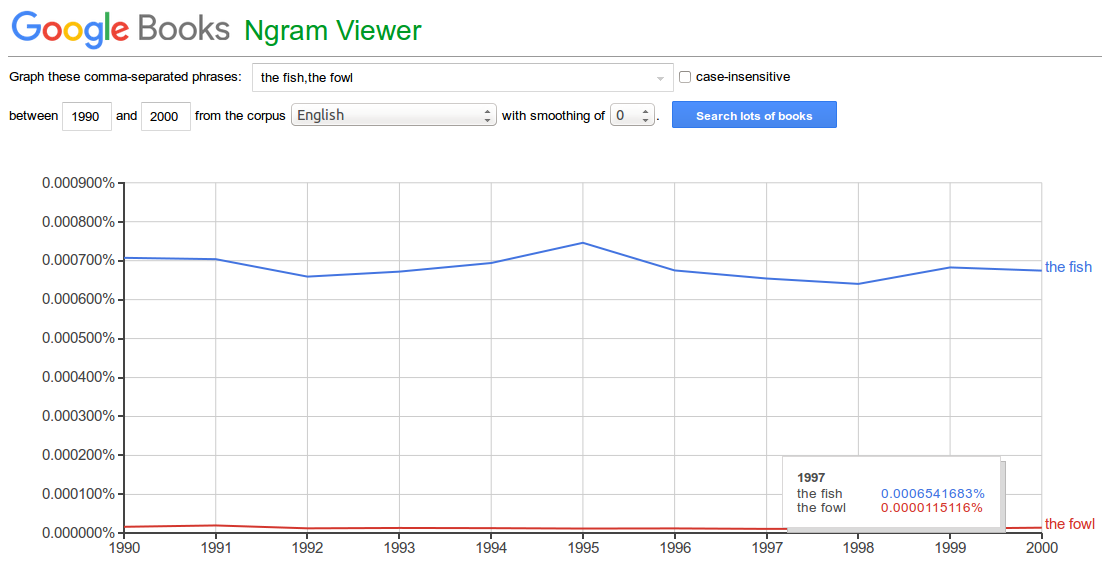
\includegraphics[width=0.75\textwidth]{../images/fishvfowl.png}
  \end{center}
}

\pagestepalt{But lots of things follow ``the''.}{
  \begin{center}
    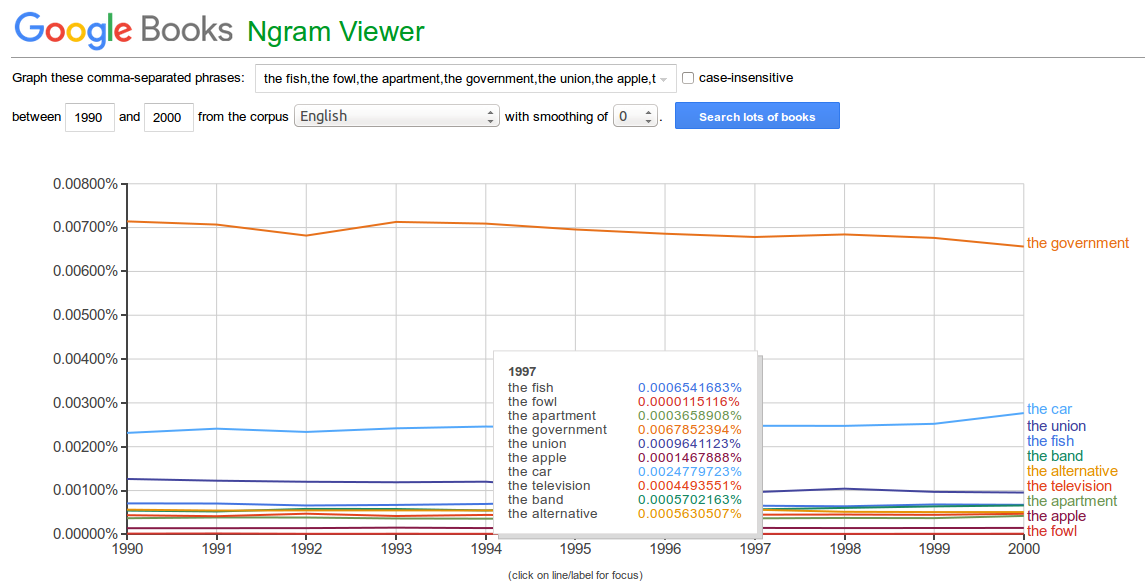
\includegraphics[width=0.8\textwidth]{../images/fishvlots.png}
  \end{center}
}

\pagestepalt{It's not hugely informative\ldots}{
  \ldots because the whole category of nouns can follow ``the''.\\ \pause
  So what if we add another word, ``eat'':
  \begin{center}
    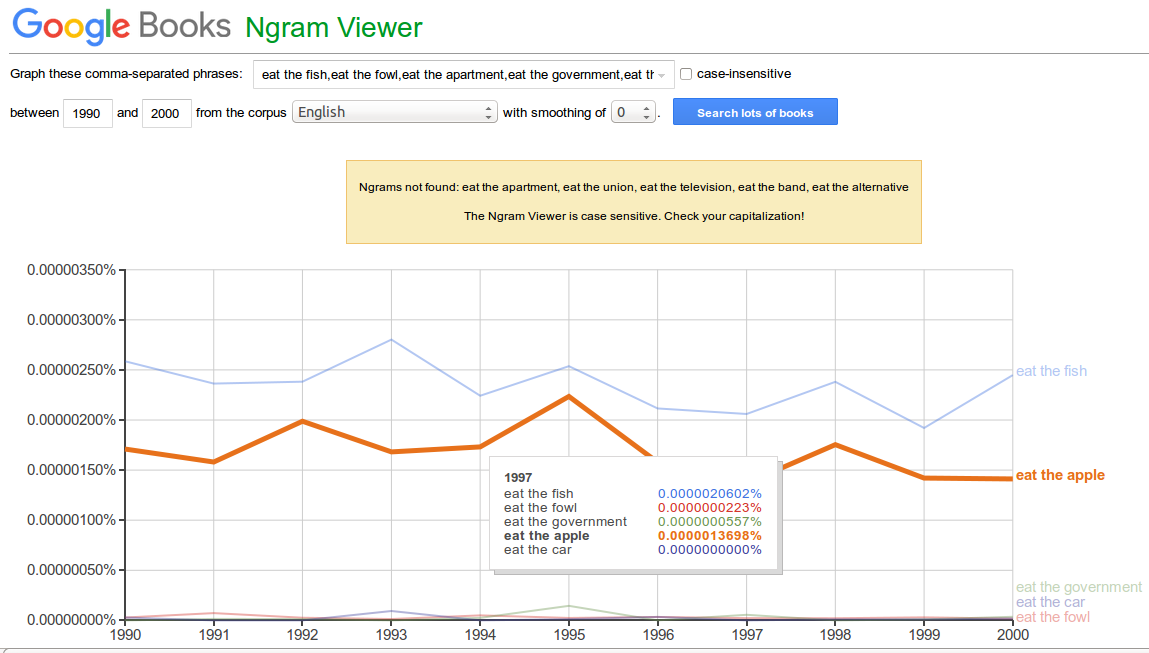
\includegraphics[width=0.75\textwidth]{../images/eat.png}
  \end{center}
}

\pagestepalt{The additional word is hugely informative!}{
  So this is a way language is \textbf{not} like the weather.\pause
  \begin{itemize}
  \item Sure, tomorrow will resemble today, in terms of temperature.
    \begin{itemize}
    \item But knowing what happened yesterday  doesn't drastically
      change the estimate.
    \end{itemize}\pause
  \item But make your \alert{{\bf bi}gram} into a \alert{{\bf tri}gram}:
    \begin{itemize}
    \item The distribution radically changes.
    \item ``eat'' is very informative.
    \end{itemize}
  \end{itemize}
}

\pagestepalt{We can even look for \alert{4-grams}.}{
  Thus we just call these \alert{$n$-grams}, for any $n$. \\
  So when we look for 4-grams starting with ``quickly eat the fish/apple/car''? \pause
  \begin{center}
    \large\textbf{Google Ngrams doesn't find anything! (for 1990-2000)}.
  \end{center}\pause
  Not even ``quickly eat the apple''!\pause
  \begin{center}
    \textbf{It's not always the case that trigrams work, but they're often practical because of \alert{sparsity}.}
  \end{center}
  
%  \textcolor{blue}{[student exercise with Google NGrams]}
}

\placard{And that involved a lot of things we're going to talk about during the rest of the course.}

\placard{Part 2: the course}

\pagestepalt{Who are we?}{
  You already know me, but:\pause
  \begin{itemize}
  \item Asad Sayeed (``course organizer'')
    \begin{itemize}
    \item Senior Lecturer with FLoV (CLASP, GRIPES projects)
    \item Ph.D., Computer Science, University of Maryland (2011).
    \item Research areas: machine learning for NLP, computational psycholinguistics, and more
    \end{itemize}\pause
  \item Vidya Somashekarappa
    \begin{itemize}
    \item Computational linguistics PhD student at CLASP
    \item Research areas: gaze analysis, neurolinguistics
    \end{itemize}
  \end{itemize}
}


\pagestepalt{Format of the course}{
  The ``rhythm'' of the course will look approximately like this, with occasional exceptions:
  \begin{itemize}
  \item Mondays: Q\&A (on any previous video lecture)
  \item Thursdays: help session for assignments
  \end{itemize}
  All content will be posted as video lectures, slides, etc on the Canvas page.
}

\pagestepalt{Evaluation of the course}{
  \begin{itemize}
  \item Deliverables (by you :) ):
    \begin{itemize}
    \item 3 assignments, including programming and problem-solving, each expected to take 2-3 weeks (can break this up based on student preference)
    \item There is \alert{\textbf{no}} final written exam.
    \end{itemize}
  \item Tentative course grade: 33\% per assignment plus 1 free percent.
  \item Tentative standard:
    \begin{itemize}
    \item Pass (G): Complete 3 assignments, obtain min 50\% on each assignment.
    \item Pass-with-distinction (VG): Complete 3 assignments, get min 90\% average overall.
    \end{itemize}
  \end{itemize}
}

\pagestepalt{Assignments}{
  \begin{itemize}
  \item Individual submission, can help each other in small groups.
  \item coding projects, \alert{mostly} Python, possibly some mathematics
  \item submission via Canvas.
  \item We will aim for 15 business days of turnaround from submission, if submitted on time.  Otherwise, latest by the summer.
  \item First assignment will be out very soon.
  \end{itemize}
}

\placard{Please review the university's academic integrity policies.}

\pagestepalt{Emphasis of the course}{
  \begin{itemize}
  \item Practical skills in statistical NLP.
    \begin{itemize}
    \item Emphasis on the data pipeline.
    \item Goal: getting from data to analysis/model/application.
    \item Gain familiarity with some statistical NLP tools.
    \end{itemize}
  \item Foundational theoretical skills.
    \begin{itemize}
    \item Getting an intuitive grasp of the mathematical underpinnings of statistical NLP techniques.
    \item Just enough for application.
    \item (Preliminary knowledge required for machine learning course in Fall!)
    \end{itemize}
  \end{itemize}
}

\pagestepalt{Tentative topic list}{
%  \vspace{-0.5cm}
  Based on how we progress (I frequently change direction based on student request/preferences/progress).
  \begin{itemize}
  \item Calculus review.
  \item More programming topics and computing skills for statistical NLP.
  \item Working with text data.
  \item Introduction to modern machine learning techniques (incl. deep learning)
  \item Applications in various areas of NLP (e.g., document classification,
    machine translation) based on an {\it ad hoc} basis.
  \end{itemize}
}

\pagestepalt{Technical details}{
  I'm assuming you have a background in basic Python programming from previous courses.
  \begin{itemize}
  \item Programming: mostly Python 3.x, using nltk, scikit-learn, pandas, and other relevant Python packages.
  \item We will introduce neural networks via PyTorch.
  \item Recommended to have your own laptop with a Linux installation, but
    we will also use mltgpu or eduserv.
  \item We will introduce git and make use of command-line techniques.
  \end{itemize}
}

\placard{This course is contiguous with the Machine Learning for NLP advanced course in the fall.}

\pagestepalt{Readings/textbook}{
  \begin{itemize}
  \item No regular readings in the beginning, this is principally a practical course.
  \item Students are encouraged to do their own research on the Internet to find clarificatory material on topics (there is a wealth of it, and it is an important skill in this business).
  \item Main textbook: ``Natural Language Processing with PyTorch'', readings will start in the middle of the course. (also used in first half of Machine Learning course)
  \end{itemize}
}

\placard{Student discussion of course desiderata}

\placard{Part 3: More (optional) boring review}

\pagestepalt{Formal Languages}{
  \vspace{-1cm}
\begin{block}{}
\begin{itemize}
	\item Once Upon a Time...
	\pause
	\item Mathematicians started to think about language...
	\pause
	\item They used ideas from logic to represent linguistic objects...
	\pause
	\item They had a really, mmm, audacious idea... \\
	\pause
	\begin{center}
	
\includegraphics[width=0.6\textwidth]{../images/doc_brown_strings.jpg}
	\end{center}
\end{itemize}
\end{block}
}


\pagestepalt{Strings}{
  \vspace{-1cm}
\begin{block}{What's a String?}
\begin{itemize}
	\item A \textbf{string} in this context is just a sequence of words
	\pause
	\item A \textbf{formal language} ($L$) is a subset of all the possible strings
	\pause
	\item An \textbf{vocabulary} ($\Sigma$, also sometimes called \textit{alphabet}) here is a set of all the words in the language
	\pause
	\item Words here don't need to correspond to words used for natural languages
	\pause
	\item For example, this set:\\
	\begin{center}
	{\LARGE \{ \Smiley[][cyan], \Springtree, \Snowman \}}\\
	\end{center}
	is a perfectly valid vocabulary for a formal language. \pause But we usually use boring symbols like \{a, b, c\}
	\pause
	\item {\scriptsize (Similar to musical/poetic form analysis)}
\end{itemize}
\end{block}
}


% Formal grammar: grammar, automaton
\pagestepalt{Formal Grammar}{
\begin{block}{}
\begin{itemize}
	\item A formal grammar is a way of telling what a valid string is in a formal language
	\item Formal grammars can also \textbf{generate} valid strings
	\pause
% weak & strong generative capacity
	\item If two different grammars can generate/accept the same formal languages, then they have the same \textbf{weak generative capacity}
	\pause
	\item If two different grammars can generate/accept the same structures as well, then they have the same \textbf{strong generative capacity}
\end{itemize}
\end{block}
}


% Chomsky Hierarchy
\pagestepalt{Formal Language Hierarchy}{
\begin{center}
\begin{tabular}{|ll|}
\hline
& Formal Language \\
\hline
\hline
& Non-Turing-acceptable\\
\hline
0: & \bf Recursively enumerable \\
\hline
& Recursive/\,Decidable \\
\hline
1: & Context-sensitive \\
\hline
& Indexed \\
\hline
& \bf Mildly context-sensitive \\
\hline
2: & \bf Context-free \\
\hline
& \bf Deterministic context-free \\
\hline
3: & \bf Regular \\
\hline
& \bf Finite \\
\hline
\end{tabular}
\end{center}
\pause
\footnotesize{This is extended from the older \textit{Chomsky hierarchy}. \pause We'll discuss the ones in boldface, as they're relevant to natural languages.}
}


% applications of knowing this stuff
\pagestepalt{Why is this Stuff Relevant??}{
\begin{block}{}
\begin{itemize}
	\item Knowing what types of formal languages a grammar/automaton can generate \& accept will give you an idea of what phenomena in natural languages that they can handle
	\pause
	\item For example: long-distance dependencies, complex reordering in machine translation, reduplication, etc.
	\pause
	\item You can also get an idea of how fast or slow it will take for a computer (or human) to process sequential stuff (like natural language!)
\end{itemize}
\end{block}
}


\pagestepalt{Finite Languages}{
\begin{block}{}
\begin{itemize}
	\item In a finite language, there are a finite (ie not infinite) number of valid \textit{sentences}.
	\item Time: constant (through hash-table lookup)
	\item Memory: constant (duh)
	\pause
	\item For natural language, this would correspond to having a finite number of possible sentences
\end{itemize}
\end{block}
}


\pagestepalt{Are Natural Languages Finite??!!}{
  \vspace{-1cm}
\begin{block}{}
\begin{itemize}
	\item It sounds rather odd to think that you could ever list all of the possible sentences of a natural language
	\pause
	\item But...
	\pause
	\item There's a big difference between a really large number and infinity
	\pause
	\item {\small If a natural language has a vocabulary of, say, 100 million words ...}
	\pause
	\item And a sentence can have, say, up to 10,000 words in it, ...
	\pause
	\item Then there would be $10^{80,000}$ possible sentences
	\pause
	\item This number sounds way too big to be practical for either humans or computers to deal with!
	\pause
	\item But it's much smaller than infinity.
	\pause
	\item Much much smaller.
	\pause
	\item \tiny{\href{http://people.umass.edu/~partee/726_04/lectures/Is_Language_Infinite.pdf}{(There's more discussion on the interwebs if you're interested)}}
\end{itemize}
\end{block}
}


\pagestepalt{(A digression on complexity)}{
  \begin{block}{}
    \begin{itemize}
    \item Processing different kinds of languages take different kinds of machines.\pause
    \item The automaton that recognizes a language represents an algorithm.\pause
    \item Algorithms take up ``space'' units (memory to process) and ``time'' units (number of steps to do something).\pause
    \item We can characterize what this means in terms of the length of the input string, which we'll call $n$.\pause
    \item Then we have something called big-$\mathcal{O}$ notation from computer science. To make a long story short:
      {\footnotesize \begin{tabular}{|l|l|l|}
        \hline
        $\mathcal{O}(1)$ & ``constant time'' & \# units unrelated to input\\
        $\mathcal{O}(n)$ & ``linear time'' & \# units lin. proportional to input string\\
        $\mathcal{O}(n^2)$ & ``quadratic time'' & {\# unites quadrat. \newline prop. to input string} \\
        \ldots &&\\
        \hline 
      \end{tabular} }
    \end{itemize}
  \end{block}
}

% Regular language: fixed history: linear time, constant memory.  Regular grammars can actually do alot
\pagestepalt{Regular Languages}{
\begin{block}{}
\begin{itemize}
	\item Ok, so maybe for now it's too difficult to list all possible sentences
	\item Let's assume that the vocabulary ($\Sigma$) is still fixed (or finite), but we can generate an infinite number of sentences from this fixed vocab
	\item Regular grammars have a fixed-length history, so they're limited in the types of long-distance phenomena they can handle
	\pause
	\item For example: $\bf a \ a^{\prime} \ b \ b^{\prime} \ c \ c^{\prime}$
	\pause
	\item Processing regular languages can be done in linear time \detail{($\mathcal{O}(n)$)}, with a constant size of memory \detail{($\mathcal{O}(1)$)}
\end{itemize}
\end{block}
}


% DCF lang: full history, as long as unambiguous: linear time, log^2(n) memory
\pagestepalt{Deterministic Context-Free Languages}{
\begin{block}{}
\begin{itemize}
	\item Deterministic context-free (DCF) languages include longer-distance phenomena
	\item DCF grammars have a full-length history, as long as there's no ambiguity (ie.\ it can't backtrack)
	\pause
	\item Processing DCF languages can be done in linear time \detail{($\mathcal{O}(n)$)}, with linear memory usage \detail{($\mathcal{O}(n)$)}
\end{itemize}
\end{block}
}


\pagestepalt{Context-Free Languages}{
\begin{block}{}
\begin{itemize}
	\item Context-free languages include phenomena like center embedding
	\item For example: $\bf a \ b \ c \ c^{\prime} \ b^{\prime} \ a^{\prime}$
	%% (use whiteboard for now to draw example)
	\pause
	\item Context-free grammars have a full-length history, and they can backtrack for ambiguous sentences
	\pause
	\item Processing CF languages can be done in about cubic time \detail{($\mathcal{O}(n^3)$)}, with linear memory usage \detail{($\mathcal{O}(n)$)}
\end{itemize}
\end{block}
}


% MCS lang: same, allows full reduplication (cross-serial deps) and a^n b^n c^n d^n: n^6 time. TAG, CCG, LIG, Head Grammars, 
\pagestepalt{Mildly Context-Sensitive Languages}{
\begin{itemize}
	\item Mildly context-sensitive (MCS) languages include phenomena like reduplication and cross-serial dependencies.
	\item Example: $\bf a \ b \ c \ a^{\prime} \ b^{\prime} \ c^{\prime}$
	\pause
	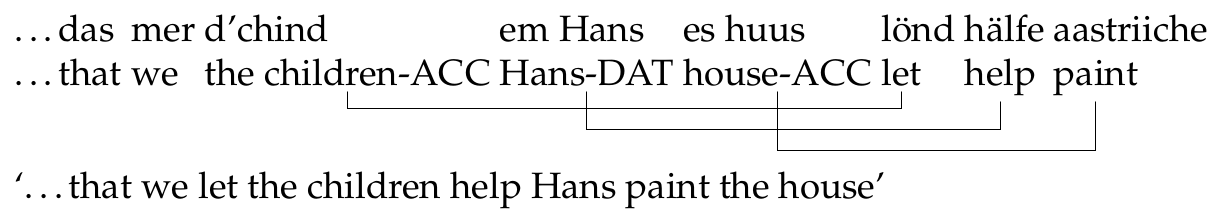
\includegraphics[width=0.80\textwidth]{../images/swiss_cross_serial_deps.png}
	%% (use whiteboard for now to draw example)
	\pause
	\item Processing MCS languages can be done in about $\mathcal{O}(n^6)$ time, with quadratic memory usage \detail{($\mathcal{O}(n^2)$)}
	\pause
	\item {\small Mildly context-sensitive is very different from context-sensitive, which is much more powerful}
	\item Some grammar formalisms that can handle MCS langs:
	\begin{itemize}
	\begin{footnotesize}
		\item \href{https://en.wikipedia.org/wiki/Tree-adjoining_grammar}{Tree Adjoining Grammar} (TAG)
		\item \href{https://en.wikipedia.org/wiki/Combinatory_categorial_grammar}{Combinatory Categorial Grammar} (CCG)
		\item \href{https://en.wikipedia.org/wiki/Indexed_grammar\#Linear_indexed_grammars}{Linear Indexed Grammars} (LIG) (easy to understand)
		\item \href{https://en.wikipedia.org/wiki/Head_grammar}{Head Grammars} (HG)
	\end{footnotesize}
	\end{itemize}
\end{itemize}
}


% Recursively enumerable langs: allows any string that a computer (eg. Turing machine, untyped \lambda calculus, MLP) can generate
\pagestepalt{Recursively Enumerable Languages}{
\begin{itemize}
	\item Recursively enumerable languages allow any string that a computer (or equivalent device) can generate/accept
	\item There's no guarantee that the computer will ever stop processing the sentence
	\item Essentially any word can occur in any place in the sentence
	\pause
	\item Some grammar formalisms that allow recursively enumerable languages include:
	\begin{itemize}
		\item \href{https://en.wikipedia.org/wiki/Transformational_grammar}{Chomskyan grammars} (due to transformations / moves)
		\item \href{https://en.wikipedia.org/wiki/Lexical_functional_grammar}{Lexical Functional Grammar} (LFG)
		\item \href{https://en.wikipedia.org/wiki/Head-driven_phrase_structure_grammar}{Head-driven Phrase Structure Grammar} (HPSG) (due to \textsc{Slash} features)
	\end{itemize}
	\pause
	\item Note that these grammar formalisms can place some restrictions on word order, but they still accept/generate recursively enumerable languages. \pause How is that so? \pause Additional grammar rules can work around such restrictions to accept/generate the string.
\end{itemize}
}

\pagestepalt{But that's just strings\ldots}{
  \vspace{-1cm}
  \begin{center}
    \href{http://science.howstuffworks.com/science-vs-myth/everyday-myths/string-theory.htm}{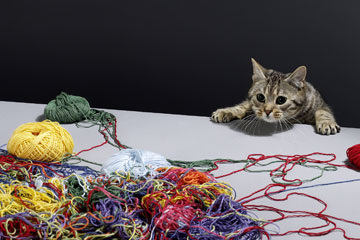
\includegraphics[width=0.5\textwidth]{../images/string-theory.jpg}}
  \end{center}\pause
  \begin{itemize}
  \item Why do we care how the strings are structured?\pause
  \item Because different structures enable different computations!\pause
  \item For example: context-free languages harder to machine-learn than regular languages.
  \end{itemize}
}

\pagestepalt{Meaning: something to do with language?}{
  \begin{center}
    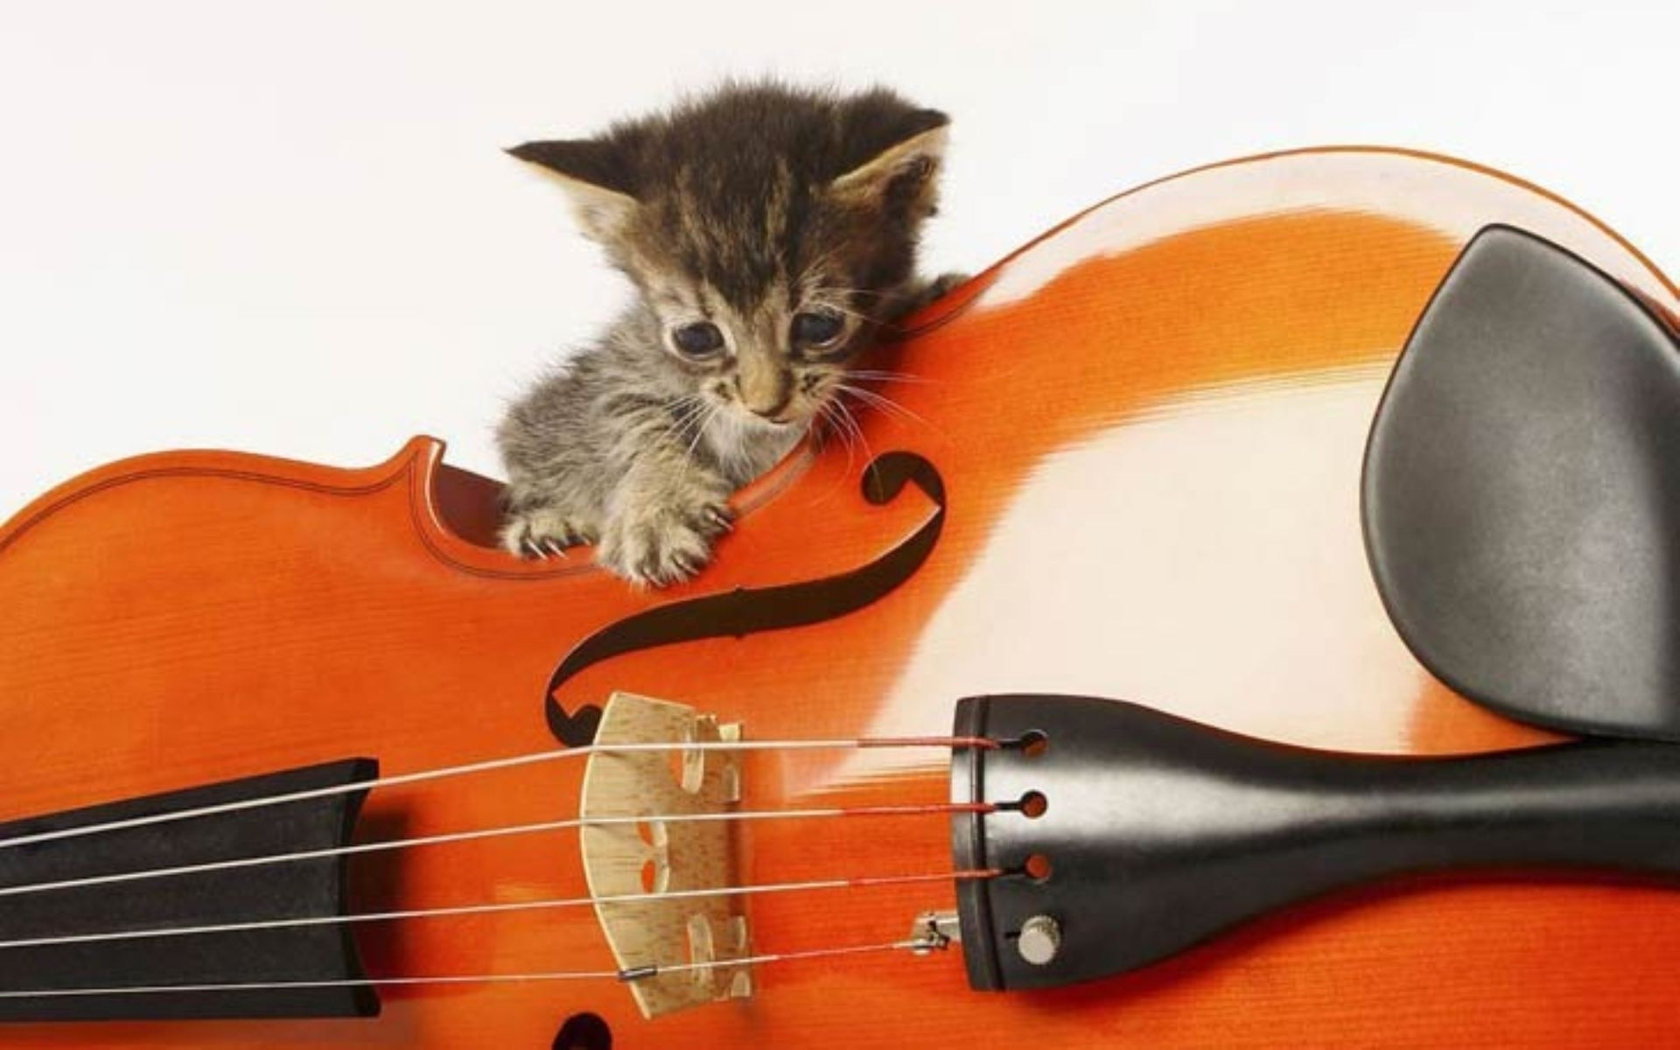
\includegraphics[width=0.4\textwidth]{../images/kitten-violin.jpg}
  \end{center}\pause
  \begin{itemize}
  \item In some sense, we want to get at the meaning in language.\pause
  \item Implicit or explicit meaning?\pause
    \begin{itemize}
    \item Machine learning: perhaps just map structures in one language to structures in another? No meaning required.\pause
    \item Computer vision -- maybe we really want explicit descriptions of objects in human language.
    \end{itemize}
  \end{itemize}
}

\pagestepalt{Lexical representation}{
  \begin{itemize}
  \item Words have meanings.  How do we describe what a word means?\pause
  \item First attempt: use ``features.'' \pause
    \begin{itemize}
    \item ``bachelor'' $=$ +male, +adult, -married\pause
    \item ``husband'' $=$ +male, +adult, +married\pause
    \item ``bachelor'' $=$ ``husband'' $\times$ (-married)\pause
    \end{itemize}
  \item Dictionary problem: what is the meaning of a feature?  Define words in terms of other words?
  \end{itemize}
}

\pagestepalt{Compositional and sentence meaning}{
  \begin{itemize}
  \item But sentences have meanings too! \pause
  \item ``The kitten is playing the violin'' -- DOER: kitten, THING DONE TO: violin, ACTION: play\pause
  \item Common way of representing this: first-order predicate calculus.\pause
    \begin{itemize}
    \item $\exists x \exists y \mathit{kitten}(x) \& \mathit{violin}(y) \& \mathit{play}(x, y)$\pause
    \item Does this really represent the meaning relationships well?\pause
    \end{itemize}
  \item The main question of formal semantics: what do we need to reason about language?
  \end{itemize}
}

\pagestepalt{To put a long story short\ldots}{
  \begin{itemize}
  \item We want to \alert{model} complex formal objects \alert{robustly}.
  \item The rest of this course is about exploiting \alert{continuous distributions of values} to do so.
  \end{itemize}
}


\end{document}
